\documentclass{beamer}

\mode<presentation>{
	%\usetheme{CambridgeUS}
	%\usecolortheme{seahorse}
	\usetheme{Boadilla}
	\usecolortheme{beaver}
	\setbeamertemplate{navigation symbols}{}
}

\usepackage{graphicx}
\usepackage{booktabs}
\usepackage{algpseudocode}
\usepackage{hyperref}
\usepackage{tikz}
\usepackage[utf8]{inputenc}
\usepackage{listings}
\usepackage[export]{adjustbox}
\usepackage{aeguill}

%\setbeamertemplate{title page}[default][rounded=false]

\setbeamertemplate{title page}
{
%\vbox{}
\begingroup
\centering
\begin{beamercolorbox}[sep=8pt,center]{institute}
\usebeamerfont{institute}\insertinstitute
\end{beamercolorbox}
\vskip1em%
\begin{beamercolorbox}[sep=8pt,center]{title}
\usebeamerfont{title}\inserttitle\par%
\ifx\insertsubtitle\@empty%
\else%
\vskip0.25em%
{\usebeamerfont{subtitle}\usebeamercolor[fg]{subtitle}\insertsubtitle\par}%
\fi%
\end{beamercolorbox}%
\vfill
\begin{beamercolorbox}[sep=8pt,center]{author}
\usebeamerfont{author}\insertauthor
\end{beamercolorbox}
\vskip1em\par
\begin{beamercolorbox}[sep=8pt,center]{date}
\usebeamerfont{date}\insertdate
\end{beamercolorbox}
\endgroup
}

\setbeamertemplate{blocks}[default]
\setbeamercolor{structure}{fg=darkred}
%\setbeamercolor{block title}{bg=darkred,fg=white}
%\setbeamercolor{block body}{bg=darkgray!20!white}
\setbeamercolor{block title}{bg=darkgray!30!white}
\setbeamertemplate{enumerate items}[default]

\setbeamertemplate{part page}{
\begin{beamercolorbox}[sep=8pt,center,wd=\textwidth]{part title}
\usebeamerfont{part title}\insertpart\par
\end{beamercolorbox}
\vfill
\tableofcontents
}

%\setbeamertemplate{frametitle continuation}{(\insertcontinuationcount)}

\setbeamertemplate{headline}{\leavevmode\hbox{\begin{beamercolorbox}[wd=.5\paperwidth,ht=2.65ex,dp=1.5ex,center]{section in head/foot}\usebeamerfont{section in head/foot}\insertsectionhead\hspace*{2ex}
\end{beamercolorbox}\begin{beamercolorbox}[wd=.5\paperwidth,ht=2.65ex,dp=1.5ex,center]{subsection in head/foot}\usebeamerfont{subsection in head/foot}\hspace*{2ex}\insertsubsectionhead\end{beamercolorbox}}\vskip0pt}

\setbeamertemplate{background}{\tikz[overlay,remember picture]\node[opacity=0.08]at (current page.south east){
\includegraphics[width=10cm]{figures/unibo_logo.jpg}};}

\newcommand{\tcc}[1]{\textcolor{darkred}{#1}}

\newcommand{\codeA}[1]{\texttt{#1}}
\newcommand{\codeB}[1]{\texttt{\textcolor{darkred}{#1}}}

\newcommand{\link}[1]{{\footnotesize » \url{#1}}}
\newcommand{\bothquote}[1]{``#1''}

\definecolor{mygreen}{rgb}{0,0.6,0}
\definecolor{mygray}{rgb}{0.5,0.5,0.5}
\definecolor{mymauve}{rgb}{0.58,0,0.82}
\definecolor{maroon}{rgb}{0.5,0,0}
\definecolor{darkgreen}{rgb}{0,0.5,0}

\lstset{
language=Java,
basicstyle=\scriptsize\ttfamily,
keywordstyle=\scriptsize\color{blue}\ttfamily,
commentstyle=\scriptsize\color{mygreen}\ttfamily,
breakatwhitespace=false,
breaklines=true,
 numbers=left,
  numberstyle=\color{mymauve},
  stringstyle=\color{mymauve},
  showstringspaces=false,
  numbers=none
}

\lstdefinelanguage{XML}
{
  basicstyle=\scriptsize\ttfamily,
  morestring=[s]{"}{"},
  morecomment=[s]{?}{?},
  morecomment=[s]{!--}{--},
  commentstyle=\color{darkgreen},
  moredelim=[s][\color{black}]{>}{<},
  moredelim=[s][\color{red}]{\ }{=},
  stringstyle=\color{blue},
  identifierstyle=\color{maroon},
  numbers=none
}

\makeatother

\AtBeginSection[]
{
  \begin{frame}
    \frametitle{Outline}
    \tableofcontents[currentsection]
  \end{frame}
}

%\AtBeginSubsection[]
%{
%  \begin{frame}
%    \frametitle{Outline}
%    \tableofcontents[currentsection,currentsubsection]
%  \end{frame}
%}

\institute[UNIBO]{\uppercase{Alma Mater Studiorum -- Università di Bologna}\\Dipartimento di Informatica -- Scienza e Ingegneria (DISI)\\C.d.S. in Ingegneria e Scienze Informatiche, Campus di Cesena}

\author[A. Marfoglia]{Alberto Marfoglia\\\scriptsize\texttt{alberto.marfoglia2@unibo.it}}


\title[Android -- 1D -- Service]{Android Programming}
\subtitle{Service}

\date[ver. 1.0 (20220505)]{Embedded Systems and Internet of Things\\A.A. 2021 -- 2022}


\begin{document}
  \begin{frame}
    \titlepage
  \end{frame}

  \newcommand\blfootnote[1]{%
  \begingroup
  \renewcommand\thefootnote{}\footnote{#1}%
  \addtocounter{footnote}{-1}%
  \endgroup
}

\begin{frame}{Thanks}
    \centering
    \begin{itemize}
      \item \large{Professor Angelo Croatti}
    \end{itemize}

    \blfootnote{\url{https://www.unibo.it/sitoweb/a.croatti/en}}
    \blfootnote{}
\end{frame}

\section{Overview}

  \begin{frame}{Service (Overview)}
    \begin{block}{Overview}
      It represents the component dedicated to the execution of
      \textit{long-running} task in the background.
      \begin{itemize}\itemsep10pt
        \item Without user interaction (there is no UI for the Services) 
      \end{itemize}
      \begin{itemize}\itemsep10pt
        \item A Service can continue its execution in the background even if the
        application that started it is stopped.
        \item From other components it is possible to request the execution of
        tasks to the Service via a special interface.
        \item There are essentially two \textit{types} of Service.
        \begin{itemize}
          \item \tcc{Started Service}
          \item \tcc{Bound Service}
        \end{itemize}
      \end{itemize}
    \end{block}
  \end{frame}

\subsection{Started Service vs. Bound Service}

  \begin{frame}{Started Service}
    \begin{block}{Fundamentals}
      \begin{itemize}\itemsep10pt
        \item It's started by another component, via an Intent passed as a
        parameter to the \codeB{startService(Intent i)} method (defined in the
        \codeA{android.app.Activity} class).
        \item It can run in the background indefinitely.
        \item Generally, it performs a specific task and return no results to the
        "father" component.
        \item At the end of the execution of its task, it terminates itself by
        calling the \codeB{stopSelf()} method (defined in the
        \codeA{android.app.Service} class) 
      \end{itemize}
    \end{block}
  \end{frame}

  \begin{frame}{Bound Service}
    \begin{block}{Fundamentals}
      \begin{itemize}\itemsep10pt
        \item It's started by another component via an Intent passed as a
        parameter to the \codeB{bindService(Intent i, ServiceConnection s, int
        flags)} function (defined in the \codeA{android.content.Context} class).
        \item It provides a Client-Server interface that allows other components
        to interact with the Service itself.
        \item The Service remains active as long as there is at least one
        component connected to it (bound).
        \begin{itemize}
          \item Several components can be connected to the Service at the same
          time but when the last one disconnects, the service is destroyed by
          the system.
        \end{itemize}
      \end{itemize}
    \end{block}
  \end{frame}

  \begin{frame}[fragile]{Service (note)}
    \begin{block}{}
      \begin{enumerate}
        \item Despite the division between \textit{Started} and \textit{Bound}
        services, the same Service can work in both modes at the same time.
        \item \textbf{Each Service runs in the Main Thread}
      \begin{itemize}
        %\item It does not create a separate thread or run in a process of its own.
        \item Therefore, if the Service has to perform CPU-intensive computation
        or blocking tasks, these must be delegated to a separate thread created
        appropriately within the Service.
      \end{itemize}
      \item Like the Activity, the Services must also be declared in the Manifest
      file in order to be identified by the system.
      \end{enumerate}
    \end{block}
    \begin{exampleblock}{}
      \begin{lstlisting}[language=XML]
<application>
<service android:name="com.example.MyService"
android:label="@string/service_name"/>
</application>
      \end{lstlisting}
    \end{exampleblock}
  \end{frame}

  \begin{frame}{Service or Thread?}
    \begin{block}{How to choose}
      \begin{itemize}\itemsep20pt
        \item Service: you must use a Service when you need to continue to perform
        the task even when the user is not interacting with the application.
        \item Thread: you must use a Thread if a relevant task is to be performed
        only while the user is interacting with the application (possibly via an
        Async Task)
      \end{itemize}
    \end{block}
  \end{frame}

\subsection{Service Lifecycle}

  \begin{frame}[allowframebreaks]{Service Lifecycle}
    \begin{itemize}\itemsep10pt
      \item Like an Activity, component Service also has its own lifecycle.
      \begin{itemize}
        \item Again, some callbacks (which can be overridden) are associated
        with state transitions.
      \end{itemize}
      \item It's not necessary to call the original version of the superclass
      when redefining the callback.
      \item In the case of the Started Service, must be redefined the
      \codeB{onCreate()}, \codeB{onStartCommand()} and \codeB{onDestroy()}
      methods.
      \item In the case of the Bound Service, must be redefined the
      \codeB{onCreate()}, \codeB{onBind()}, \codeB{onUnbind()} and
      \codeB{onDestroy()} methods.
    \end{itemize}
    \begin{figure}
      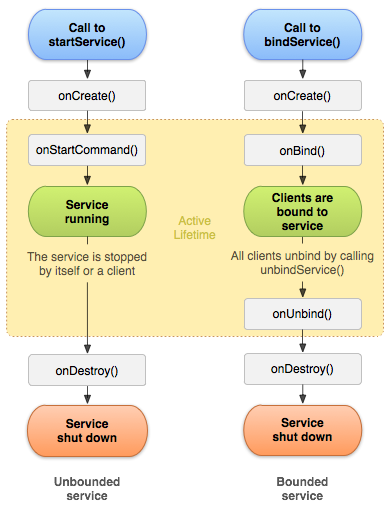
\includegraphics[width=0.48\linewidth]{figures/service_lifecycle.png}
    \end{figure}
  \end{frame}

  \begin{frame}[allowframebreaks]{Service Lifecycle -- Callback}
    \begin{block}{\codeB{void onCreate()}}
      \begin{itemize}
        \item Invoked after the creation of the Service. 
      \end{itemize}
    \end{block}

    \begin{block}{\codeB{int onStartCommand(Intent i, int flags, int startId)}}
      \begin{itemize}
        \item Invoked after the creation of the Service, if the creation has
        been requested through the \codeA{startService()} function.
      \end{itemize}
    \end{block}

    \begin{block}{\codeB{void onDestroy()}}
      \begin{itemize}
        \item Invoked before the system destroys the Service no longer used.
      \end{itemize}
    \end{block}

  \framebreak

    \begin{block}{\codeB{IBinder onBind(Intent i)}}
      \begin{itemize}
        \item Invoked after connecting a component to the Service through the
        \codeA{bindService()} function.
        \item It returns an object instance of type \codeA{IBinder} that allows
        the caller to interact with the Service.
      \end{itemize}
    \end{block}

    \begin{block}{\codeB{boolean onUnbind(Intent i)}}
      \begin{itemize}
        \item Invoked after a component (previously connected to the Service)
        has decided to disconnect through the \codeA{unbindService()} function.
      \end{itemize}
    \end{block}
  \end{frame}

\section{Started Service Management}
  \begin{frame}[fragile]{Creation and Boot of a Started Service}
    \begin{block}{Steps}
      \begin{enumerate}\itemsep10pt
        \item You need to instantiate an object that extends from the
        \codeB{android.app.Service} class.
        \item The component that creates the service must prepare a specific
        Intent and invoke the \codeB{startService(Intent i)} method to start the
        Service.
      \end{enumerate}
    \end{block}
    \begin{exampleblock}{Exmaple}
      \begin{lstlisting}[language=Java]  		        
Intent i = new Intent(this, MyService.class);
startService(i); // fires the onStartCommand() method
      \end{lstlisting}
    \end{exampleblock}
  \end{frame}

\subsection{Intent Service}
  \begin{frame}{Intent Service}
    \begin{block}{IntentService -- semplified approach}
      The \codeB{android.app.IntentService} class extends from \codeA{Service} and
      makes it much easier to create a Started Service.
      \begin{itemize}\itemsep10pt
        \item You must define a constructor that invokes the parent one, passing a
        name for the worker thread that will be associated automatically to the
        Service.
        \item You must redefine the \codeB{onHandleIntent(Intent i)} method, which
        is invoked when the service starts.
        \item Additionally, when the method terminates, the service terminates as well.
      \end{itemize}
    \end{block}
  \end{frame}

  \begin{frame}[fragile]{Intent Service - Example}
    \begin{exampleblock}{Example}
      \begin{lstlisting}[language=Java]  		        
public class MyService extends IntentService {

  public MyService() {
    super("MyServiceWorkerThread");
  }

  @Override
  protected void onHandleIntent(Intent intent) {
    //do something
  }
}
      \end{lstlisting}
    \end{exampleblock}
    \textbf{NOTE}: The redefinition of the other callbacks requires the explicit
    invocation of the same of the superclass.
  \end{frame}

\section{Bound Service Management}
  \begin{frame}[fragile]{Creation of a Bound Service}
    \begin{block}{BoundService}
      \begin{itemize}\itemsep10pt
        \item You must create an instance of an object that extends the
        \codeB{android.app.Service} class.
        \item The component that creates the service must prepare a specific
        Intent and invoke the \codeB{bindService(Intent i, ServiceConnection sc,
        int flags)} method to start the Service.
      \end{itemize}
    \end{block}
    \begin{exampleblock}{Example}
      \begin{lstlisting}[language=Java]
  ServiceConnection conn = ... ;
  Intent i = new Intent(this, MyBoundService.class);
  bindService(i, conn, Context.BIND_AUTO_CREATE);
      \end{lstlisting}
    \end{exampleblock}
    \small You must set up an appropriate communication channel (\tcc{binder}) that
     allows you to interact with the service
  \end{frame}

  \begin{frame}{Bound Service Lifecycle (Details)}
    \begin{figure}
      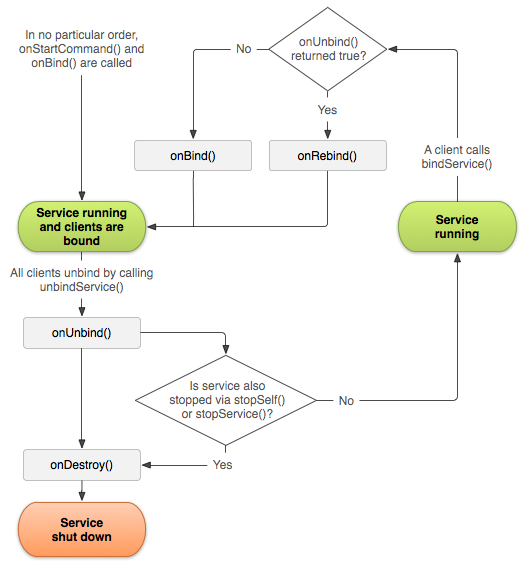
\includegraphics[width=0.56\linewidth]{figures/service_bound_lifecycle.png}
    \end{figure}
  \end{frame}

\subsection{Binder use case}

  \begin{frame}[fragile,allowframebreaks]{Bound Service with Binder -- Example}
    Goal: {\footnotesize \textit{We want to create a service that provides a
    random number to the connected components in response to specific requests}}
    \begin{exampleblock}{Example -- Definition of a Service}
      \begin{lstlisting}[language=Java]
public class RndGenService extends Service {
  private final IBinder binder = new RndGenBinder();
  private final Random generator = new Random();

  @Override
  public IBinder onBind(Intent intent) {
    return binder;
  }
  
  /* RandomGenService API methods */
  public int getRandomNumber() {
    return generator.nextInt(100);
  }
      \end{lstlisting}
    \end{exampleblock}  
    \begin{exampleblock}{\vspace{-10pt}}
      \begin{lstlisting}[language=Java]
  /* Binder for the RndGenService */
  class RndGenBinder extends Binder {
    public RndGenService getService() {return RndGenService.this;}
  }
}
      \end{lstlisting}
    \end{exampleblock}

    \begin{itemize}
      \item The \codeA{onBind()} method must return the instance of an object of
      type \codeB{IBinder} appropriately defined as the inner-class of the
      service.
      \begin{itemize}
        \item This object (\codeA{RandomGenBinder}, in the example) must expose
        a public method (\codeA{getService()}) that returns the instance of the
        service to which the binder belongs.
      \end{itemize}
      \item Finally, the API of the service must be defined, i.e. the methods
      that can be invoked from outside (\codeA{getRandomNumber()}, in the
      example).
    \end{itemize}

    \begin{exampleblock}{Example -- Activity using the Service}
      \begin{lstlisting}[language=Java]
public class MyActivity extends Activity {
  private RndGenService service;
  private boolean bounded = false;

  private ServiceConnection conn = new ServiceConnection() {
    @Override
    public void onServiceConnected(ComponentName cls, IBinder bnd){
      service = ((RndGenService.RndGenBinder) bnd).getService();
      bounded = true;
    }

    @Override
    public void onServiceDisconnected(ComponentName cls) {
      bounded = false;
    }
  };
      \end{lstlisting}
    \end{exampleblock}  
    \begin{exampleblock}{\vspace{-10pt}}
      \begin{lstlisting}[language=Java]   
  @Override
  protected void onCreate(Bundle savedInstanceState){/*...*/}

  @Override
  protected void onStart() {
    super.onStart();
    Intent intent = new Intent(this, RndGenService.class);
    bindService(intent, conn, Context.BIND_AUTO_CREATE);
  }

  @Override
  protected void onStop(){
    super.onStop();
    if(bounded){
      unbindService(conn);
      bounded = false;
    }
  }
      \end{lstlisting}
    \end{exampleblock}  
    \begin{exampleblock}{\vspace{-10pt}}
      \begin{lstlisting}[language=Java]
  public void onButtonClick(View v) {
    if(bounded){
      int nextRndNum = service.getRandomNumber();
    }
  }
}
      \end{lstlisting}
    \end{exampleblock}
      \begin{itemize}
        \item The binding of the service is possible by defining an object of type
        \codeB{android.content.ServiceConnection} that establishes and maintains
        the connection between the activity and the service.
        \item For that object you must define the following methods:
        \begin{itemize}
          \item \codeB{onServiceConnected()}: allows to retrieve the service
          reference using the Binder (inner class of the service) and its
          \codeA{getService()} method. 
          \begin{itemize}
            \item Through this reference it's possible to invoke the Service API.
          \end{itemize}
          \item \codeB{onServiceDisconnected()}  
        \end{itemize}
        \item Method \codeB{bindService()} is passed both the Intent for creating the service and
        the object representing the connection.
        \item The service can be released by calling the \codeB{unbindService()}
        method, passing the connection reference as a parameter.
      \end{itemize}
    \end{frame}

    \begin{frame}{Bound Service with Binder -- Notes}
      \begin{block}{Notes}
        \begin{itemize}\itemsep20pt
          \item The explicit use of a Binder is allowed only when the component
          that wants to use the service belongs to the same application.
          \item Otherwise, the \tcc{Messenger-based} mechanism must be used, which allows
          you to request the execution of methods defined in services of other
          processes/applications.
          \begin{itemize}
            \item That is, when it is not possible to have an explicit reference
            to the Service instance object. 
          \end{itemize}
        \end{itemize}
      \end{block}
  \end{frame}

\subsection{Messenger use case}

  \begin{frame}[fragile,allowframebreaks]{Bound Service with Messenger -- Example}
    \begin{exampleblock}{Example -- Definition of the Messaging Service}
      \begin{lstlisting}[language=Java]
public class MessengerService extends Service {
  static final int MESSAGE_1_REQUEST = 1;
  static final int MESSAGE_2_REQUEST = 2;
  
  final Messenger m = new Messenger(new IncomingHandler());
  
  @Override
  public IBinder onBind(Intent intent) {
    return m.getBinder();
  }

  private class IncomingHandler extends Handler {
    @Override
    public void handleMessage(Message msg) {
      switch(msg.what) {
        case MESSAGE_1_REQUEST:
          //do something
      \end{lstlisting}
    \end{exampleblock}  
    \begin{exampleblock}{\vspace{-10pt}}
      \begin{lstlisting}[language=Java]
          break;
        case MESSAGE_2_REQUEST:
          //do something
          break;
        default:
          super.handleMessage(msg);
          break;
      }
    }
  }
}
      \end{lstlisting}
    \end{exampleblock}

    \begin{itemize}
      \item The service defines an \codeB{android.os.Messenger} object as internal
      field.
      \begin{itemize}
        \item Initialized using a Handler specifically designed to receive
        messages from calling components
      \end{itemize}
      \item The \codeA{onBind()} method returns the reference to the binder
      obtained directly from the Messenger instance.
    \end{itemize}

    \begin{exampleblock}{Esempio -- (external) Activity that uses the Service}
      \begin{lstlisting}[language=Java]
public class ActivityMessenger extends Activity {
private Messenger service = null;
private boolean bounded;

private ServiceConnection conn = new ServiceConnection() {
  public void onServiceConnected(ComponentName cls, IBinder bnd) {
    service = new Messenger(bnd);
    bounded = true;
  }
  
  public void onServiceDisconnected(ComponentName cls) {
    service = null;
      \end{lstlisting}
    \end{exampleblock}  
    \begin{exampleblock}{\vspace{-10pt}}
      \begin{lstlisting}[language=Java]    
      bounded = false;
    }
  };

  @Override
  protected void onCreate(Bundle savedInstanceState) {
    /* ... */
  }

  @Override
  protected void onStart(){
    super.onStart();
    
    Intent i = new Intent(this, MessengerService.class)
    bindService(i, conn, Context.BIND_AUTO_CREATE);
  }
      \end{lstlisting}
    \end{exampleblock}  
    \begin{exampleblock}{\vspace{-10pt}}
      \begin{lstlisting}[language=Java]
  @Override
  protected void onStop() {
    super.onStop();

    if(bounded) {
      unbindService(conn);
      bounded = false;
    }
  }

  public void requireServiceMessage1(View v) {
    if (!bounded) return;
    
    Message msg = Message.obtain(null, MessengerService.MESSAGE_1_REQUEST, 0, 0); 
    try { service.send(msg); } 
    catch(RemoteException e) { /* ... */ }
  }
}    
      \end{lstlisting}
    \end{exampleblock}
  \end{frame}

\section*{References}
%-----------------------
%--- ONLINE RESURCES ---
%-----------------------

\begin{frame}{References - Online Resources}
\begin{thebibliography}{99}
\setbeamertemplate{bibliography item}[online]

\bibitem{adAPIguide} Android Developers - Guide
\newblock \link{https://developer.android.com/guide/}

\bibitem{adAPIreference} Android Developers - API Reference
\newblock \link{https://developer.android.com/reference/}

\bibitem{adTraining} Android Developers - Samples
\newblock \link{https://developer.android.com/samples/}

\bibitem{adTraining} Android Developers - Design \& Quality
\newblock \link{https://developer.android.com/design/}

\end{thebibliography}
\end{frame}

%-----------------------
%--- BOOKS -------------
%-----------------------

%\begin{frame}{Riferimenti - Libri}
%\begin{thebibliography}{99}
%\setbeamertemplate{bibliography item}[book]
%
%\bibitem{Mednieks11} Zigurd Mednieks, Laird Dornin, G. Blake Meike, Masumi Nakamura
%\newblock \emph{Programming Android}
%\newblock O'Reilly, 2011
%
%\bibitem{Haseman13} Chris Haseman, Kevin Grant
%\newblock \emph{Beginning Android Programming: Develop and Design}
%\newblock Peachpit Press, 2013
%
%\bibitem{Schwarz13} Ronan Schwarz, Phil Dutson, James Steele, Nelson To
%\newblock \emph{The Android Developer's Cookbook : Building Applications with the Android SDK}
%\newblock Addison-Wesley, 2013 
%
%\bibitem{Neil14} Theresa Neil
%\newblock \emph{Mobile Design Pattern Gallery: UI Patterns for Smartphone App}
%\newblock O'Relly, Second Edition, 2014
%\end{thebibliography}
%\end{frame}

\end{document}
